\documentclass[
    iai & comatec, % Saisir le nom de l'institut rattaché
    mi, % Saisir le nom de l'orientation
    %confidential, % Décommentez si le travail est confidentiel
]{heig-tb}

\usepackage[nooldvoltagedirection,european,americaninductors]{circuitikz}
\usepackage{comment}
\usepackage{caption}
\usepackage{subcaption}
\usepackage{pdfpages}
\usepackage{multicol}


\signature{ThaoNhi.svg} % Remplacer par votre propre signature vectorielle.

\makenomenclature
\makenoidxglossaries
\makeindex

\addbibresource{bibliography.bib}

\input{nomenclature}
\input{acronyms}

\newglossaryentry{heig-vd}{
    name=HEIG-VD,
    description={Haute École d'Ingénierie et de Gestion du canton de Vaud}
}
\newglossaryentry{hes-so}{
    name=HES-SO,
    description={Haute École Supérieure de Suisse Occidentale}
}
\newglossaryentry{latex}{
    name=latex,
    description={Un langage et un système de composition de documents}
}
\newglossaryentry{maths}{
    name=mathematics,
    description={Les mathematiques sont ce que les mathématiciens fonts}
}

\newglossaryentry{capteur}{
    name=FUN,
    description={\textbf{F}l\textbf{u}xmètre \textbf{N}anoporeux (capteurs de débit)}
}

\newglossaryentry{infrarouge}{
    name=IR,
    description={acronyme pour infrarouge, rayonnement électromagnétique d'une certaine longueur d'onde (entre 780nm et 1mm)}
}

\newglossaryentry{pvd}{
    name = PVD,
    description = {Physical Vapor Deposition ou dépôt physique en phase vapeur, procédé de métallisation qui permet de déposer des fines
            couches d'un certain métal}
}

% Auteur du document (étudiant-e) en projet de Bachelor
\author{Thao Nhi LA}

% Activer l'option pour l'accord du féminin dans le texte
\genre{female}

% Titre de votre travail de Bachelor
\title{Débimètre respiratoire pédiatrique} %\LaTeX~de rapport de Bachelor

% Le sous titre est optionnel
\subtitle{Travail de Bachelor}

% Nom du professeur responsable
\teacher {Prof. Laurent Gravier (HEIG-VD)}

% Mettre à jour avec la date de rendu du travail
\date{\today}

% Numéro de TB
\thesis{7212}



\surroundwithmdframed{minted}

%% Début du document
\begin{document}
\selectlanguage{french}
\maketitle
\frontmatter
\clearemptydoublepage

%% Requis par les dispositions générales des travaux de Bachelor
\preamble
\authentification

%% Résumé / Résumé publiable / Version abrégée
\begin{abstract}
    % Francais
Dans le domaine de la santé, les nouveau-nés sont des patients requérant des soins très spécifiques, et tout particulièrement en cas de 
naissance prématurée. Un monitoring précis de leurs paramètres vitaux est alors indispensable pour permettre au personnel médical d'effectuer 
les soins les plus adaptés. Parmi ces paramètres le monitoring du débit respiratoire est primordial. Cependant, les très petits volumes 
pulmonaires ainsi que des fréquences respiratoires élevées pousse les appareils conventionnels à leurs limites de détection. L'objectif de ce 
projet est de prouver la faisabilité d'un débitmètre par nanotechnologie. Un tel débitmètre assurerait un temps de réponse absolument prometteur pour 
un prix relativement faible. 

\asterism

La technologie derrière ce débitmètre repose sur l'effet Seebeck, phénomène extrêmement connu dans les thermocouples. Lorsque deux matériaux 
conducteurs ou semi-conducteurs sont associés et soumis à des températures différentes, une tension va être produite entre ces deux matériaux. \\
Le débitmètre respiratoire pédiatrique peut être assimilé à deux thermocouples fonctionnant par effet Seebeck avec un corps de chauffe inclus. 
Quand un flux d'air viendra souffler sur le corps de chauffe, un gradient de température se formera et une tension apparaîtra. Par la très faible 
taille associée aux nanotechnologies, ce type de dispositif assure un temps de réponse extrêmement faible comparé aux appareils actuels. \\

\asterism

Un banc de test a été réalisé afin de pouvoir prouver la faisabilité d'un tel capteur. Ce banc de test permet de tester les échantillons constituant 
le capteur par nanotechnologie avec différents paramètres. 


\end{abstract}

%% Sommaire et tables
\clearemptydoublepage
{
    \tableofcontents
    \let\cleardoublepage\clearpage
    \listoffigures
    \let\cleardoublepage\clearpage
    \listoftables
    \let\cleardoublepage\clearpage
    \listoflistings
}

\printnomenclature
\clearemptydoublepage
\pagenumbering{arabic}

\label{glossaire}
\printnoidxglossary

%% Contenu
\mainmatter
\chapter{Introduction}
%L'introduction est une section requise dans un rapport technique. Introduisez votre travail, l'idée de départ et les objectifs attendus. Un lecteur qui découvrirait votre projet au travers de cette introduction devrait ainsi être capable d'en comprendre le cadre, l'idée générale et les aboutissants du projet.
Dans le cadre des études à la HEIG-VD, un travail de Bachelor et demandé en fin d'études. Ce dernier représente un projet sur un semestre. 

\section{Contexte}
%Cette section \underline{n'est pas obligatoire}, mais elle est souvent présente dans un rapport technique pour compléter l'introduction et définir le contexte du travail \cad le cadre formel dans lequel le travail est mené.
Dans le domaine de la santé, les nouveau-nés sont des patients requérant des soins très spécifiques, et tout particulièrement en cas de 
naissance prématurée. Un monitoring précis de leurs paramètres vitaux est alors indispensable pour permettre au personnel médical d'effectuer 
les soins les plus adaptés. Parmi ces paramètres le monitoring de l'assistance respiratoire est doublement utile : d'une part, il permet le 
contrôle précis de cette assistance en cas de détresse respiratoire, et d'autre part la mesure du débit respiratoire couplé au taux d'oxygène 
et de dioxyde de carbone donne des informations précieuses sur l'énergie dépensé par ces petits organismes. Cependant, les très petits volumes 
pulmonaires ainsi que des fréquences respiratoires élevées pousse les appareils conventionnels à leurs limites de détection. Des appareils plus 
adaptés à ces contraintes doivent être développés, qui d'une part doivent drastiquement minimiser les volumes morts qui fausse l'estimation du 
volume pulmonaire, et d'autre part doivent avoir une réponse temporelle très rapide. 

Ce travail de Bachelor porte sur la faisabilité d'un débitmètre respiratoire par nanotechnologie, qui mesurerait le flux d'air entrant et 
sortant sans volume mort et avec un temps de réponse inférieure à 100 ms. 

Ce projet vise ainsi à fabriquer des débitmètres par nanotechnologie et de développer un banc de test ad hoc pour en mesurer les performances.  

\section{Objectifs}
Ce travail de Bachelor vise à démontrer la faisabilité de débitmètre respiratoire utilisant des capteurs élaborés par une nanotechnologie à 
faibles coûts. Il se décline en quatre objectifs pratiques : \\
\vspace{0.2cm}
\textbf{Objectif 1} - Élaboration d'un cahier de spécifications \& d'un catalogue de solutions. \\
\vspace{0.2cm}
\textbf{Objectif 2} - Conception et réalisation d'un débitmètre par nanotechnologie. \\
\vspace{0.2cm}
\textbf{Objectif 3} - Conception et réalisation d'un banc de test dédié au débitmètre.\\
\vspace{0.2cm}
\textbf{Objectif 4} - Qualification des performances du débitmètre.

\section{État de l'art}
\subsection{Débitmètres néonatals sur le marché}
Plusieurs entreprises proposent des débitmètres néonatals. Ces entreprises ont été regroupées dans le tableau ci-dessous avec les 
technologies de capteur utilisées. \\
\begin{table}[H]
    \centering
    \begin{tabular}{|c|c|}
        \hline
        \textbf{Entreprises} & \textbf{Technologie}                \\
        \hline
        Sensirion            & Capteur thermique de débit massique \\
        \hline
        Mim-Germany          & Anémomètre à fil chaud double       \\
        \hline
        Europlaz             & Anémomètre à fils chauds            \\
        \hline
        Draeger              & Anémomètre à fil chaud              \\
        \hline
    \end{tabular}
    \caption{Débitmètres pédiatriques sur le marché}
    \label{tab:debitmetreMarche}
\end{table}


\subsection{Revues scientifiques}
Les revues scientifiques sont également des ressources intéressantes à considérer pour l'élaboration de l'état de l'art. En effet, les 
articles scientifiques vont permettre d'établir une liste des techniques déjà exploitées, leur fonctionnement détaillé ainsi que leurs 
performances. \\
\begin{figure}[H]
    \hspace{-1cm}
    \includegraphics[scale = 0.45]{images/DRP_Etat_de_l_art.png}
    \caption{Articles scientifiques par ordre chronologique}
    \label{fig:articlesChrono}
\end{figure}

Les articles pertinents pour ce Travail de Bachelor sont résumés dans ce chapitre et classé par ordre chronologique sur la figure 
\ref{fig:articlesChrono}. \\

Les principales technologies exploitées comme débitmètre pédiatrique sont passée en revue ci-dessous. 

\subsubsection{Effet de Venturi}
Le débit respiratoire est mesuré grâce à une différence de pression. Cette différence de pression est engendré par un rétrécissement de 
l'espace de circulation du gaz (principe de Venturi) \cite{oberg_biomedical_2011}. 
\begin{figure}[H]
    \centering
    \includegraphics[scale = 0.5]{assets/figures/Venturi.png}
    \caption{Effet de Venturi \cite{oberg_biomedical_2011}}
    \label{fig:venturi}
\end{figure}

La figure \ref{fig:venturi} illustre l'effet Venturi. Avec un rétrécissement de la partie centrale d'un tube, le fluide traversant le dispositif 
sera accéléré et subira également une dépression à cet endroit. Ainsi, en mesurant la pression à différents endroits du tube, il est possible 
de calculer le flux d'air. \\

C'est la technologie utilisée par les pneumotachographes (le pneumotachographe de Fleisch par exemple). Mais elle peut également être utilisée 
dans une application quelque peu différente. En effet, un article mentionne son utilisation dans un ressuscitateur \cite{jacq_ultra-low_2011}. 
Un tel appareil permet la réanimation du patient qui ne respire plus. Le ressuscitateur gonfle les poumons d'air et ainsi s'assure qu'un bon 
taux d'oxygène circule dans le patient. \\
Pour les nouveaux-né, la quantité d'air injectée dans les poumons doit être mesurée, car un trop grand débit pourrait rapidement engendrer 
des dégâts. \\
Couplé au système de Venturi, un capteur de force vient mesurer la pression et le volume d'air passant par le ressuscitateur. \\

Cette technologie a l'avantage d'être connue et utilisée depuis maintenant longtemps. Elle offre alors une certaine confiance aux utilisateurs. 
De plus, elle procure un débit linéaire. \\
Cependant, elle possède le désavantage d'être sensible aux conditions environnementales. Un thermostat est donc souvent nécessaire \cite{fischberg_pratique_2009}.

\subsubsection{Anémomètre à fils chauds}
Par la suite, il est expliqué que le pneumotachographe est gentiment remplacé par les anémomètres à fil chaud. Ces capteurs sont 
constitués d'un ou plusieurs fils chauffés par une source de courant. Lorsqu'un flux d'air va souffler sur le fil, ce dernier va être refroidi. 
Le niveau de refroidissement est directement lié au débit du flux \cite{oberg_biomedical_2011}. \\
L'article susmentionné conseil l'utilisation des anémomètres à deux fils contrairement à ceux à un seul fil qui aurait des performances 
moindres. 
L'anémomètre à fils chauds est une technologie incorporée par exemple dans la machine "Draeger Babylog", marque mentionnée dans le tableau \ref{tab:debitmetreMarche}. \\

L'avantage de cette technologie est qu'elle possède une faible résistance intrinsèque et est moins sensible à l'environnement. Toutefois, les 
filaments sont plus fragiles et deux filaments sont nécessaires pour des questions de fiabilité du résultat. 

\subsubsection{Transfert de chaleur entre deux transistors}

Une autre technologie pour débitmètre consiste à utiliser le transfert de chaleur entre deux transistors. 
\begin{figure}[H]
    \centering
    \includegraphics[scale = 0.5]{images/Debitmetre_transistors.png}
    \caption{Principe du débitmètre à transistors\cite{giorgino_design_2014}}
    \label{fig:transistors}
\end{figure}

C'est un principe encore innovant décrit dans l'article \cite{giorgino_design_2014}, utilisé dans l'article \cite{rosi_device_2016} et illustré 
par la figure \ref{fig:transistors}. 
Le premier transistor (appelé Front transistor) est placé perpendiculairement au flux d'air sur un PCB. \\
Le second (Rear transistor) est fixé de l'autre côté du PCB, dos à dos avec le premier transistor (cf. figure \ref{fig:transistors}) et mesure la 
chaleur émise par le Front transistor et transférée par le flux d'air. \\
De cette manière, le capteur sera capable de distinguer une expiration d'une inspiration. Le temps de réponse d'un tel capteur serait 
d'environ 340 ms. C'est un très bon temps de réponse en comparaison des capteurs médicaux existants sur le marché. Cependant, diverses améliorations 
doivent encore être faites avant de pouvoir utiliser une telle technologie. 

\begin{comment}
L'article suivant est intéressant au niveau du listage des débitmètres pédiatriques existants \cite{}. En effet, il étudie les différents fonctionnements 
existants et compare les signaux obtenus. Étant donné que cet article étudie plus précisément une caractéristique ("IN-line" vs "Flow-Through"), 
il est moins important dans le cadre de ce projet.\\
\end{comment}

\subsubsection{Caméra}
La thématique de l'article \cite{villarroel_non-contact_2019} repose sur une technologie de monitoring non invasive. Elle utilise une caméra qui suit les mouvements du nouveaux-né. 
Cette technologie permet également d'enregistrer d'autres signaux tels que la fréquence cardiaque, mais elle requiert encore quelques améliorations 
ainsi que quelques recherches supplémentaires. \\

Cette technologie a le grand avantage d'être non invasive, mais n'est pas encore aboutie. 

\subsubsection{Mesure thermique par l'entreprise Sensirion}
L'entreprise Sensirion propose une technologie basée sur des mesures de températures. Une membrane incorporée dans une puce est utilisé comme 
capteur de débit. Un flux d'air vient transférer la chaleur du corps de chauffe placé au milieu de la membrane. Deux capteurs de température 
sont placés en aval et en amont du corps de chauffe, en direction du flux. Un signal précis engendré par la différence de température en aval et  
en amont sera finalement mesurable. 
\begin{figure}[H]
    \centering
    \includegraphics[scale = 0.15]{assets/figures/Sensirion_tech.png}
    \caption{Technologie proposée par Sensirion\cite{noauthor_smart_nodate}}
    \label{fig:sensirion}
\end{figure}

\subsubsection{Nanotechnologie}
Un autre article mentionne les membranes nanoporeuses comme capteur \cite{moharamzadeh_fabrication_2018}. Bien que cette technique se rapproche 
de notre application, ces capteurs sont pour l'humidité et non le débit respiratoire. Des nanostructures d'oxyde de Zinc sont utilisées, car 
elles possèdent de bonnes propriétés physiques et chimiques. Étant donné que l'humidité et le débit respiratoire sont en lien, l'article évoque 
également le débit, cependant, il ne l'étudie pas plus en détail. \\
Toutefois, un temps de réponse plutôt bon, de l'ordre de la seconde est attendu avec une telle technologie. 

\section{Benchmarking}
Avec les différentes informations récoltées de l'état de l'art, un benchmarking peut être élaboré. Ce dernier est composé de différentes valeurs 
de performance à atteindre dans l'idéal. 

\begin{table}[H]
    \centering
    \begin{tabular}{|c|c|}
        \hline
        \textbf{Plage de débit}           & $\pm 8$ l/min     \\
        \hline
        \textbf{Sensibilité de détection} & < 0.1 l/min       \\
        \hline
        \textbf{Temps de réponse}         & < 340 ms          \\
        \hline
        \textbf{Fréquence de respiration} & entre 0.3 et 3 Hz \\
        \hline
        \textbf{Diamètre des conduits}    & < 10 mm           \\
        \hline
    \end{tabular}
    \caption{Benchmarking}
    \label{fig:benchmarking}
\end{table}


\section{Fonctionnement du débitmètre respiratoire pédiatrique}
Ce travail de Bachelor est donc une recherche à propos d'un débitmètre dont le principe de fonctionnement est encore innovant. \\

Le capteur développé repose sur le phénomène de l'effet Seebeck, phénomène que l'on peut également retrouver dans les thermocouples. L'effet 
Seebeck est le suivant :\\

Lorsqu'un matériau conducteur ou semiconducteur est soumis à un gradient de température, les électrons libres vont se déplacer du chaud vers le 
froid : une tension s'établit alors entre les extrémités du matériau (Figure \ref{fig:Seebeck}\cite{instrumentys_effet_2021}).
\begin{figure}[H]
    \centering
    \includegraphics[scale = 0.3]{images/Seebeck.jpg}
    \caption{Effet de Seebeck}
    \label{fig:Seebeck}
\end{figure}

La tension est calculée grâce à la formule suivante :
\[V = S \cdot (T_{chaude} - T_{froide})\]
Avec S, le coefficient Seebeck de l'ordre de quelques $\upmu$V/K\\

Le principe du débitmètre nanostructuré est illustré sur la figure \ref{fig:schema_coupe} : un corps de chauffe est encadré par deux vias de nanofils 
thermoélectriques formants chacun un thermocouple. Un flux d'air déportera la chaleur de façon à refroidir un thermocouple et réchauffer l'autre. La 
différence de température indiquée par la tension Seebeck permettra de déduire le débit du flux d'air. De la très faible inertie thermique des 
structures nanofils est attendue une réponse temporelle très rapide. 
\begin{figure}[H]
    \centering
    \includegraphics[scale = 0.4]{images/CapteurFUN.png}
    \caption{Schéma de principe du débitmètre nanostructuré}
    \label{fig:schema_coupe}
\end{figure}

\section{Livrables}
\begin{itemize}
    \item Cahier de spécifications
    \item Débitmètre fonctionnel
    \item Banc de test
    \item Rapport technique
\end{itemize}

\newpage
\section{Planification}
\begin{table}[H]
    \centering
    \begin{tabular}{lllllllll}
                                                                                                                  &                                                                               &                                                                               &                                                                               &                                                                               &                                                                               &                       &  & \\ \cline{2-9}
        \multicolumn{1}{l|}{}                                                                                     & \multicolumn{1}{c|}{\begin{tabular}[c]{@{}c@{}}23.02 - \\ 23.03\end{tabular}} & \multicolumn{3}{c|}{\begin{tabular}[c]{@{}c@{}}23.03 - \\ 09.05\end{tabular}} & \multicolumn{1}{c|}{\begin{tabular}[c]{@{}c@{}}09.05 - \\ 08.06\end{tabular}} & \multicolumn{2}{c|}{\begin{tabular}[c]{@{}c@{}}15.06 - \\ 13.07\end{tabular}} & \multicolumn{1}{c|}{\begin{tabular}[c]{@{}c@{}}13.07 - \\ 27.07\end{tabular}}                              \\ \hline
        \multicolumn{1}{|l|}{\begin{tabular}[c]{@{}l@{}}Prise en main du projet \\ et état de l'art\end{tabular}} & \multicolumn{1}{l|}{\cellcolor[HTML]{9AFF99}}                                 & \multicolumn{3}{l|}{}                                                         & \multicolumn{1}{l|}{}                                                         & \multicolumn{2}{l|}{}                                                         & \multicolumn{1}{l|}{}                                                                                      \\ \hline
        \multicolumn{1}{|l|}{\begin{tabular}[c]{@{}l@{}}Formation à l'électro-\\ déposition\end{tabular}}         & \multicolumn{1}{l|}{}                                                         & \multicolumn{2}{l|}{\cellcolor[HTML]{9AFF99}}                                 & \multicolumn{1}{l|}{}                                                         & \multicolumn{1}{l|}{}                                                         & \multicolumn{2}{l|}{}                                                         & \multicolumn{1}{l|}{}      \\ \hline
        \multicolumn{1}{|l|}{\begin{tabular}[c]{@{}l@{}}Conception du support du \\ capteur\end{tabular}}         & \multicolumn{1}{l|}{}                                                         & \multicolumn{1}{l|}{}                                                         & \multicolumn{3}{l|}{\cellcolor[HTML]{9AFF99}}                                 & \multicolumn{2}{l|}{}                                                         & \multicolumn{1}{l|}{}                                                                                      \\ \hline
        \multicolumn{1}{|l|}{Rendu intermédiaire}                                                                 & \multicolumn{1}{l|}{}                                                         & \multicolumn{3}{l|}{}                                                         & \multicolumn{1}{l|}{}                                                         & \multicolumn{1}{l|}{\cellcolor[HTML]{9AFF99}}                                 & \multicolumn{1}{l|}{}                                                         & \multicolumn{1}{l|}{}      \\ \hline
        \multicolumn{1}{|l|}{Conception du banc de test}                                                          & \multicolumn{1}{l|}{}                                                         & \multicolumn{3}{l|}{}                                                         & \multicolumn{1}{l|}{}                                                         & \multicolumn{2}{l|}{\cellcolor[HTML]{9AFF99}}                                 & \multicolumn{1}{l|}{}                                                                                      \\ \hline
        \multicolumn{1}{|l|}{Mesures}                                                                             & \multicolumn{1}{l|}{}                                                         & \multicolumn{3}{l|}{}                                                         & \multicolumn{1}{l|}{}                                                         & \multicolumn{1}{l|}{}                                                         & \multicolumn{2}{l|}{\cellcolor[HTML]{9AFF99}}                                                              \\ \hline
        \multicolumn{1}{|l|}{Rapport}                                                                             & \multicolumn{8}{l|}{\cellcolor[HTML]{D3FDD3}}                                                                                                                                                                                                                                                                                                                                                                                              \\ \hline
    \end{tabular}
\end{table}

L'avancée du travail a été suivie par une séance hebdomadaire. 

\section{Plan du rapport}
La présentation du travail effectué est structurée en cinq chapitres distincts :
\begin{description}
    \item[Chapitre 1 -] Cahier des spécifications\\
        Revue de la littérature, rédaction d'un état de l'art et définition du benchmarking. \\
    \item[Chapitre 2 -] Conception et réalisation du capteur nanostructuré\\
        Électrodéposition, déposition physique en phase vapeur (\gls{pvd}), conditionnement du capteur (réalisation des supports)\\
    \item[Chapitre 3 -] Conception et réalisation du banc de test\\
        Commandes, études des différents composants du banc de test, réalisation, montage et validation\\
    \item[Chapitre 4 -] Qualification du capteur\\
        Définition d'un protocole de mesures, résultats et analyses\\
    \item[Chapitre 5 -] Conclusion\\
\end{description}


%\input{examples.tex}

\chapter{Fabrication des capteurs FUNs}
\section{Catalogue des solutions}
Plusieurs systèmes ont été étudiés afin d'incorporer le capteur dans une conception permettant de connecter les membranes et le corps de chauffe
ainsi que d'y attacher un système apportant un flux d'air (imitation de la respiration du patient).

\subsection{Design 1}
\begin{figure}[H]
    \centering
    \includegraphics[scale = 0.3]{images/Design1.png}
    \caption{Design 1}
    \label{fig:design1}
\end{figure}
Ce premier design est le plus basique. Il vient plaquer le capteur entre deux couches presque semblables. Sur une des couches se trouvent des
perçages permettant de tenir des contacts à ressorts (pointes ressorts). Celles-ci viennent s'appuyer d'un côté sur le capteur et
de l'autre, une  connection pourra être faite par des pinces crocodiles ou des soudures. \\
Un joint plat peut venir de part et d'autre du capteur afin d'assurer l'étanchéité du système.\\
Cette solution a le désavantage d'avoir une arrivé d'air scindée en deux. Le placement ainsi que l'étanchéité au niveau de l'entrée
d'air risque d'être mauvaise. \\
Ceci mis de côté, c'est une solution simple, rapide et compacte.

\subsection{Design 2}
Afin d'éviter l'entrée d'air scindée en deux, une solution pourrait être celle représentée ci-dessous :
\begin{figure}[H]
    \centering
    \includegraphics[scale = 0.3]{images/Capteur_design2_caoutch.png}
    \caption{Design 2}
    \label{fig:design2}
\end{figure}
L'arrivée d'air se fait par le haut du système et est dévié par la suite afin d'arriver sur le capteur. Cette solution permet d'avoir une
entrée d'air plus régulière et utilisable que la solution précédente. Cependant, elle ajoute un risque non-négligeable au niveau des turbulences. En effet,
les coudées risquent d'engendrer des turbulences au niveau du flux qui pourraient altérer les résultats.\\
Une particularité à noter est le fait que la membrane se retrouve entièrement plaquée contre une surface contrairement à la solution
précédante où le centre de la membrane (là où est situé le capteur), "flotte" au milieu du flux d'air.

\subsection{Design 3}
Une manière de diminuer les turbulences seraient d'élargir le système afin que les coudées ne se retrouvent pas trop proches de la
membrane.

\begin{figure}[H]
    \centering
    \includegraphics[scale = 0.3]{images/Design4}
    \caption{Design 3}
    \label{fig:design4}
\end{figure}

\begin{comment}
\section{Design 4}
Une autre manière d'éviter ce problème de turbulences et de changer la conception. Ainsi, le capteur pourrait être fabriqué selon la
figure \ref{fig:design6}.

\section{Design 4}%à effacer
\begin{figure}[H]
    \centering
    \includegraphics[scale = 0.5]{images/Design6}
    \caption{}
    \label{fig:design6}
\end{figure}

Cependant cette solution engendre un nombre de pièces plus élevé que les designs précédents. En effet, pour un conception comme celle
de la figure \ref{fig:design6}, 4 pièces seraient nécessaires contre 2 pièces pour les solutions précédentes.\\
Deux pièces viendraient pincer le capteur en sandwich comme montré pour le design 1, figure \ref{fig:design1}, puis, deux autres pièces
viendraient se poser sur les deux longueurs du système afin de permettre de conncter facilement une arrivée d'air.
\end{comment}

\subsection{Design 4}
Finalement, une dernière conception a été imaginée :
\begin{figure}[H]
    \centering
    \includegraphics[scale = 0.4]{images/Design5_int_caoutch.png}
    \caption{Design 4}
    \label{fig:design5}
\end{figure}

Cette dernière permettrait de garder une solution à deux pièces seulement et incorporerait une entrée et une sortie d'air facilitée
(non-scindée en deux).\\
La membrane (capteur) posée sur une première pièce légèrement surrélevée. Un joint plat d'échantéité viendrait sur la membrane (en noir
sur la figure). Puis, une seconde pièce viendrait s'appuyer en sandwich contre le joint et le capteur. Cette pièce, sur le dessus, est
percée afin d'amener le flux d'air au niveau du capteur. Des plus petits perçages ainsi que des espaces creusés dans la pièce du dessus
permettent aux pointes ressorts de venir se poser sur la membrane afin d'assurer la connection électrique.\\

Finalement, deux designs ont été retenus. Le Design 1 ainsi que le Design 5. Ces deux designs vont être testés afin de mesurer la
performance d'un capteur recevant un flux d'air depuis le haut et depuis le bas simultanément ainsi qu'un capteur ne recevant un flux
d'air seulement par le haut (car le capteur est plaqué contre une surface).

\chapter{Banc de test}

\section{Présentation}
Le banc de test correspond au système composé du capteur \gls{capteur} et des appareils des mesures. Pour ce banc de test, le matériel suivant est utilisé :
\begin{itemize}
    \item \textbf{Capteur avec son support (Design 1 ou 5)}\\
          La géométrie générale du Design 1 et 5 est expliquée et représentée au chapitre \ref*{chap:catalogueSol}. \\
          
    \item \textbf{Débitmètre de référence FESTO SFAH-10B-Q6S-PNLK-PNVBA-M8}\\
          Le débitmètre choisi est un débitmètre bidirectionnel avec une entrée d'air de 6 mm de diamètre. Il sera placé juste avant l'entrée du flux
          d'air dans le capteur, permettant ainsi d'avoir une valeur de référence fiable.\\
          
          Un graphe de la tension en fonction du débit fourni par le débitmètre de référence a été construit grâce à la sortie analogique de ce dernier :
          \begin{figure}[H]
              \centering
              \includegraphics[scale = 0.4]{assets/figures/Calibration_maison.jpg}
              \caption{Tension en fonction du débit}
              \label{fig:calibration}
          \end{figure}
          
          Sur la figure \ref{fig:calibration}, nous pouvons observer la tension mesurée en fonction d'un certain débit d'air. Les paramètres utilisés
          pour cette calibration sont les suivants :
          \begin{itemize}
              \item Sortie analogique en tension sur une plage de 0 V à 10 V
              \item Full Scale allant de 0\% à +100\%
          \end{itemize}
          
          Le graphe montre une fonction linéaire qui se rapproche très fortement de la fonction $y = x$ (f$_{mesur\acute{e}}(x) = 1.0004x - 0.0038$).\\
          
    \item \textbf{Électrovanne FESTO MHE3-MS1H-3/2G-QS-6-K}\\
          Cette électrovanne fonctionne avec une tension de 24 V.  Elle permet de créer un flux d'air pulsé. Ce flux d'air pulsé alimentera le
          capteur \gls{capteur}.\\
          Cet appareil possède 3 ports de connexion et 2 commutations différentes (également dit : vanne à 3/2 voies) disposées selon le schéma ci-dessous :
          \begin{figure}[H]
              \centering
              \includegraphics[scale = 0.3]{assets/figures/Electrovanne_InOutput.png}
              \caption{Entrée et sortie de l'électrovanne}
              \label{fig:electrovanne_InOutput}
          \end{figure}
          Les entrées/sorties sont représentées par les numéros 1, 2 et 3. L'électrovanne est représentée par deux carrés accolés (cf. figure
          \ref*{fig:electrovanne_InOutput}). Le carré de gauche montre le système au repos. Le carré de droite représente la deuxième position de
          l'électrovanne, lorsque celle-ci est mise sous tension \cite{mimwebsite}.\\
          
    \item \textbf{Transistor MOSFET IRL540N}\\
          Le MOSFET (metal-oxide-semiconductor field-effect transistor) est un transistor fonctionnant en tension. Dans notre cas, il va
          être utilisé comme un interrupteur qui va alimenter ou non l'électrovanne.
          \begin{figure}[H]
              \centering
              \includegraphics[scale = 0.05]{assets/figures/mosfet_visuel.jpg}
              \caption{MOSFET}
              \label{fig:mosfet}
          \end{figure}
          
    \item \textbf{Arduino Nano}\\
          L'Arduino Nano est un circuit-imprimé qui va également participer à la création du flux d'air pulsé. C'est grâce à l'arduino que la
          fréquence du flux d'air sera modulable. En effet, ce composant va contrôler le MOSFET, qui transmettra ensuite les informations à
          l'électrovanne.\\
          Le code utilisé afin de créer une sortie en tension par pulsation est fourni en annexe. Il a été réalisé sur le logiciel Arduino IDE.\\
          
\end{itemize}

Toutes les Datasheet des composants utilisés et achetés se trouvent en annexe. Ces Datasheet contiennent toutes les valeurs et schéma nécessaire
au dimensionnement du banc de test.

\section{Modélisation du banc de test}
\subsection{Flux d'air pulsé}
Une première solution est d'amener un flux d'air pulsé sur la membrane. Ce flux d'air serait contrôlé par une électrovanne et un
transistor MOSFET IRL540N. Ce transistor a été choisi, car il permet d'être contrôlé grâce à un Arduino Nano. En effet, sa tension de seuil
($V_{GS}$) est de 4 V, 5 V ou 10 V. Étant donné que l'Arduino Nano sortira une tension de 5 V, cette valeur sera suffisante pour faire fonctionner
le MOSFET.
\begin{figure}[H]
    \centering
    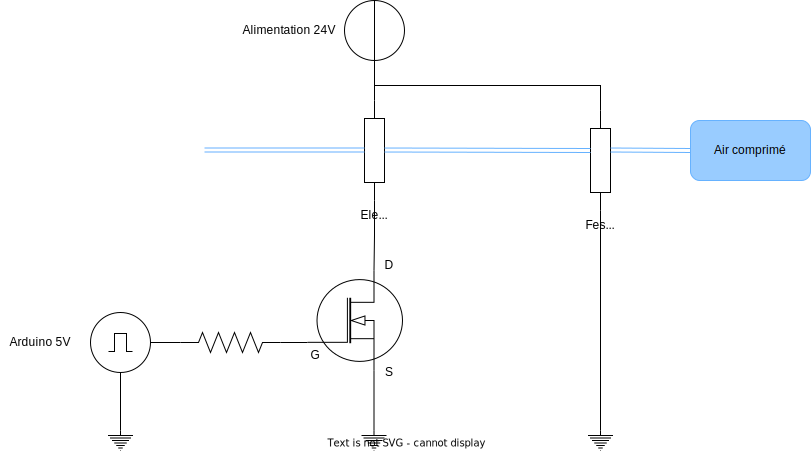
\includegraphics[scale=0.6]{assets/figures/MOSFET.png}
    \caption{Schéma électrique avec MOSFET}
    \label{fig:MOSFET}
\end{figure}
Un contrôle de la chaleur dégagée par effet Joule est utile afin de décider si un dissipateur thermique est nécessaire. Ce calcul se fait
de la manière suivante :\\
D'abord, calculons la chaleur dégagée (puissance par effet Joule) :

\[I_{electrovanne} = \frac{P_{electrovanne}}{U} = \frac{6.5}{24} \cong 0.27 \text{ A} \]
\[P_{effetJoule} = R_{DS}\cdot I^2\]
Avec :\\
$R_{DS}$ (résistance entre les jonctions D et S du MOSFET) = 0.053 $\Omega$

Ainsi :
\begin{equation}
    P_{effetJoule} = 0.053\cdot 0.27^2 \cong 3.86 \text{ mW}
\end{equation}

Les différentes valeurs de résistances, puissances, etc. se trouvent dans la datasheet du MOSFET qui se trouve en annexe. \\

Puis, nous pouvons calculer la puissance maximum dissipée par le MOSFET :
\[P_{max\,dissip\acute{e}e} = \frac{max(T_j) - T_A}{R_{\theta JA}} = \frac{175-25}{62}\cong 2.42 \text{ W}\]
Avec :\\
$T_j$ = température de jonction [\textdegree C]\\
$T_A$ = température ambiante [\textdegree C]\\
$R_{\theta JA}$ = résistance thermique, de jonction à ambiant [$\Omega$]

Ainsi, comme $P_{effetJoule} < P_{max\,dissip\acute{e}e}$, un dissipateur thermique n'est pas nécessaire. \\

Au niveau du fonctionnement général du système, le transistor est commandé par un Arduino Nano qui alimente le MOSFET avec 5 V par pulsation (1 seconde à 5 V et 1 seconde à 0 V). \\
Lorsque le MOSFET reçoit 5V, il s'active et "laisse passer" le courant qui permet à l'électrovanne de s'ouvrir et de faire passer le
flux d'air.
\begin{figure}[H]
    \centering
    \begin{subfigure}[b]{0.45\textwidth}
        \hspace{-1.5cm}
        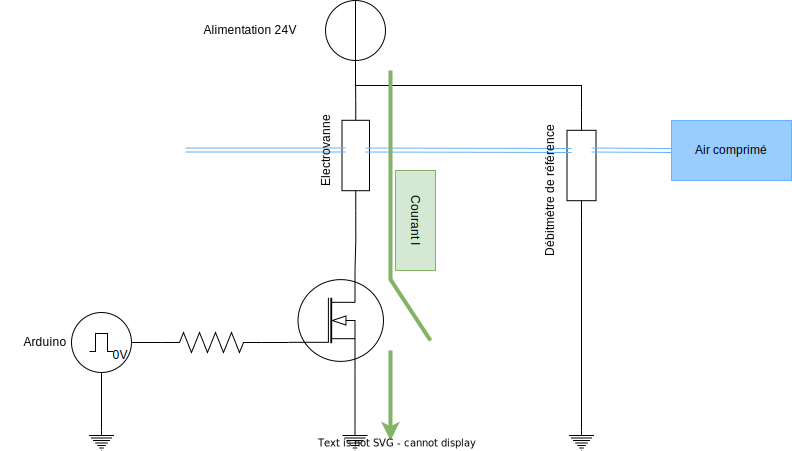
\includegraphics[scale = 0.3]{assets/figures/MOSFET_0V.png}
        \caption{MOSFET non alimenté}
        \label{fig:MOSFET_0V}
    \end{subfigure}
    \begin{subfigure}[b]{0.45\textwidth}
        \centering
        \includegraphics[scale = 0.3]{assets/figures/MOSFET_5V.png}
        \caption{MOSFET alimenté}
        \label{fig:MOSFET_5V}
    \end{subfigure}
    \caption{Fonctionnement du flux d'air pulsé}
    \label{fig:flux_pulse}
\end{figure}

Le corps de chauffe, constitué d'une fine couche d'or, doit être alimenté avec un certain courant. Ce courant, s'il est trop élevé, va abîmer la
membrane, mais s'il est trop bas, il sera insuffisant pour entraîner une différence de température de part et d'autres du capteur. \\

Le calcul suivant a don été effectué afin de déterminer le courant à utiliser pour le corps de chauffe :
\[P_{max} = R\cdot I^2\]
Avec :\\
$P_{parSurface}$ (puissance max par unité de surface) = 100 $\frac{\text{W}}{\text{m}^2}$\\
$R$ (résistance du corps de chauffe) = 45 $\Omega$\\

La valeur de puissance par unité de surface a été tirée de la puissance maximale utilisée pour les chauffages du marché (chauffage au sol).
Elle permet d'avoir un ordre de grandeur pour la valeur de courant à fournir au corps de chauffe.
La surface du corps de chauffe a été approximée à 80 mm$^2$ (2 mm $\cdot$ 40 mm).\\
Ainsi une règle de 3 a été effectuée afin de trouver la valeur de puissance pour le corps de chauffe concerné :
\[P_{max} = 8\cdot 10^{-5}\cdot 100 = 1.78\cdot 10^{-4} \text{ W}\]
\[I = \sqrt{\frac{P_{max}}{R}} = \sqrt{\frac{1.78\cdot 10^{-4}}{45}} \cong 13\text{ mA}\]
Plusieurs tests ont été alors effectué dans une plage de 10 mA à 20 mA. Ces tests ont donné un courant maximum à 15 mA. Au-delà, la membrane
est abîmée (couche d'or rongée).\\

\subsection{Conception 3D et réelle du banc de test}
\begin{figure}[H]
    \centering
    \includegraphics[scale = 0.5]{assets/figures/Banc_de_test.png}
    \caption{Conception 3D du banc de test}
    \label{fig:3D_banc_test}
\end{figure}

\subsection{Corps de chauffe pulsé}
Une autre manière de tester les capteurs \gls{capteur} serait de faire pulser le corps de chauffe et d'amener un flux d'air constant. \\
Cela signifie qu'il faut alimenter le corps de chauffe un certain temps, puis couper l'alimentation. Ceci peut se faire, comme pour l'arrivée
d'air pulsé, par un relais, un transistor tel le MOSFET ou un générateur de fonction. \\

Pour ce projet, un générateur de fonction a été utilisé afin de simplifier le processus. Ce générateur de fonction sortait un signal carré
d'une certaine tension (dépendante de la résistance du corps de chauffe) avec un offset permettant d'avoir un front descendant autour des
0 V. La tension était choisie en fonction de la résistance du corps de chauffe et du courant souhaité (ici 15 mA). En utilisant la loi d'Ohm
$U = R\cdot I$, la tension est facilement calculée.

\section{Vérification du banc de test}
La première version du banc de test est pratique, car lors de la mise en pratique, le flux d'air pulsé est aisément vérifiable. \\
Cependant, lors des premiers tests, aucun signal n'était visible sur l'oscilloscope. Ceci peut être dû à différentes raisons :
\begin{itemize}
    \item Un mauvais contact avec les pointes ressorts\\
          
    \item La puissance du corps de chauffe n'est pas suffisante\\
          
    \item L'échantillon (capteur \gls{capteur}) est défectueux\\
\end{itemize}

Afin de vérifier quel-s paramètre-s entraîne-nt un mauvais résultat, une première décision a été de tester le \gls{capteur} ouvert (sans son support,
en utilisant seulement la membrane).
Des pinces plates viennent faire le contact électrique directement sur les couches d'or afin de mesurer la tension y circulant.
\begin{figure}[H]
    \centering
    \includegraphics[scale = 0.05]{assets/figures/CapteurOuvert.jpg}
    \caption{Tests sur capteur ouvert}
    \label{fig:capteurOuvert}
\end{figure}
Cette installation ne communiquait pas non plus de résultat concluant (tension oscillant autour des 0 V). \\

Le corps de chauffe a donc été mis en question. Une alternative à ce corps de chauffe a été de venir toucher la pince plate d'un côté du
capteur afin d'engendrer une différence de température entre les deux parties coudées. Ceci a bel et bien entraîné une différence de
température et donc, une tension. Cependant, cette dernière provient de la différence de température entre l'or (sur la membrane) et le métal
de la pince plate. \\

Afin de chauffer une des deux parties électrodéposées, une court tube a été utilisé. Un flux d'air chaud a été soufflé directement sur cette
partie afin de créer un gradient de température, mais à nouveau, aucune fluctuation n'a été perçue. Cependant, lorsque le flux d'air chaud
était soufflé au niveau de la pince plate, une plus grande fluctuation de tension était visible. Cela signifie que la jonction avec le tellure
de bismuth est probablement pathologique.\\

Il était tout de même nécessaire et intéressant de vérifier si le banc de test fonctionnait de manière appropriée. Pour cela, un autre capteur
a été utilisé afin de vérifier la fonctionnalité du banc de test. \\
Le capteur utilisé est un capteur infrarouge par nanotechnologie qui traduit un certain rayonnement électromagnétique en tension. Ainsi lorsque l'on souffle
dessus, un changement dans l'environnement, et plus précisément dans la température ambiante, aura lieu. Ce flux d'air impacte donc
les rayonnements thermiques qui, eux, sont étroitement liés, entre autres, aux rayonnements infrarouges. C'est donc pour cette raison qu'à
l'oscilloscope, une fluctuation sur la tension se dessine.
\begin{figure}[H]
    \centering
    \begin{subfigure}[b]{0.45\textwidth}
        \hspace{-1 cm}
        \includegraphics[scale = 0.45]{assets/figures/CapteurIR_1s_1s.PNG}
        \caption{Air pulsé pendant 1 s puis repos pendant 1 s}
        \label{fig:1s1s}
    \end{subfigure}
    \begin{subfigure}[b]{0.45\textwidth}
        \centering
        \includegraphics[scale = 0.45]{assets/figures/1_8s_repos.PNG}
        \caption{Air pulsé pendant 1 s puis repos pendant 1.8 s}
        \label{fig:1_8s}
    \end{subfigure}
    \caption{Résultats avec capteur infrarouge}
    \label{fig:capteurIR}
\end{figure}

Les figures ci-dessus (\ref{fig:capteurIR}), montrent que le banc de test et plus précisément, le système de flux d'air pulsé accompagné de
la sortie à l'oscilloscope (en passant par l'amplificateur) fonctionne bien. En effet, sur les figures \ref*{fig:1s1s} et \ref*{fig:1_8s}
les différentes pulsations sont bien visibles.\\

Sur la figure \ref{fig:1s1s}, la récupération du capteur est plus longue que le temps de repos. C'est pourquoi le temps de repos a été allongé
et fixé à 1.8 s (figure \ref*{fig:1_8s}). Ceci permet au capteur de se remettre à zéro et permet aussi de contrôler que la fréquence est bien
modulable. \\

Une autre partie intéressante à étudier est l'amplificateur. Pour ce faire, un petit programme LabView a été utilisé afin de mesurer, dans un
premier temps, la réponse du capteur \gls{infrarouge} sans amplificateur, puis, dans un second temps, la réponse avec amplificateur. Ceci nous
permettra de qualifier l'amplificateur.

Ces tests prouvent que le banc de test semble fonctionner de manière correcte. L'échantillon est alors certainement le facteur engendrant de
mauvais résultats. Un développement de cette thématique sera effectué dans le chapitre \ref{chap:mesures}.

\newpage
\section{Mise en place du banc de test}
\begin{enumerate}
    \item Brancher l'alimentation 24 V au banc de test :
          \begin{itemize}
              \item Connecter le pôle positif de l'alimentation à une des broches de l'électrovanne
              \item Connecter le pôle négatif de l'alimentation à la broche S du MOSFET par le Jumper Wire blanc (il s'agit de la connexion à la terre)
          \end{itemize}
          
    \item Connecter le débitmètre de référence à l'alimentation :
          \begin{itemize}
              \item Connecter le câble marron du débitmètre au pôle positif de l'alimentation (par exemple, grâce à un câble sortant de l'alimentation
                    avec une pince crocodile au bout, lier la broche de l'électrovanne et le fil marron du débitmètre)
              \item Le câble bleu du débitmètre doit être lié à la broche S du MOSFET par le biais du bornier à vis sur la Breadboard
          \end{itemize}
          
          
    \item Brancher le deuxième brin de l'électrovanne à la broche D du MOSFET par le bornier à vis\\
          
    \item Brancher l'amplificateur à une alimentation secteur\\
          
    \item Brancher l'Arduino Nano à un ordinateur et lancer le programme\\
          
    \item Placer le capteur :
          \begin{itemize}
              \item Connecter le corps de chauffe et l'alimentant de maximum 15 mA. Une alimentation de laboratoire peut être utilisée en connectant
                    les deux pointes ressorts concernées par le corps de chauffe à l'alimentation de 15 mA. Les pointes ressorts pour le corps de chauffe
                    sont représentées en jaune sur la figure \ref*{fig:pointes_ressorts_chauffe}.
                    \begin{figure}[H]
                        \centering
                        \begin{subfigure}[b]{0.45\textwidth}
                            \includegraphics[scale = 0.3]{assets/figures/pointes_ressorts_chauffe.png}
                        \end{subfigure}
                        \begin{subfigure}{0.45\textwidth}
                            \includegraphics[scale = 0.3]{assets/figures/pointes_ressorts_chauffe_design5.png}
                        \end{subfigure}
                        \caption{Pointes ressorts du corps de chauffe}
                        \label{fig:pointes_ressorts_chauffe}
                    \end{figure}
          \end{itemize}
          
          
    \item Si l'amplificateur est utilisé : Connecter les deux pointes ressorts restantes à l'amplificateur grâce aux câbles sortant en haut
          à droite du banc de test\\
          
    \item Si l'amplificateur n'est pas utilisé : Connecter directement les deux pointes ressorts restantes à l'appareil de mesure utilisé
\end{enumerate}


\chapter{Mesures}

\section{Dépandances}
\section{Discussion}

\chapter{Conclusion}
\section{Conclusion générale}
Pour conclure, ce Travail de Bachelor consiste en une première étude sur les débitmètres respiratoires pédiatriques par nanotechnologie. \\
Tout d'abord, il a été prouvé et affirmé que ce type de dispositif reste assurément utile et efficace dans le domaine du diagnostic médical. 
En effet, il permet de suivre la respiration de près et d'avertir diverses maladies telles que les apnées et/ou les détresses respiratoires. \\
De plus, étant donné le caractère prometteur des nanotechnologies sur le temps de réponse ainsi que la sensibilité, une rapidité remarquable 
est attendue par ce type de dispositif. Ces avantages sont particulièrement décisifs chez les prématurés, patients dont les poumons sont encore 
fragiles et donc, sujets à diverses maladies pulmonaires.\\
Un nouveau capteur de débit a alors été développé. Sa réponse à divers environnements a été mesurée et testée afin d'en apprendre davantage sur 
ce type de débitmètre. Pour ce faire, un banc de test a été réalisé. Ce banc de test permet de souffler un flux d'air mesurable dans 
le capteur, puis d'obtenir la réponse du dispositif sur un programme LabView (graphe tension en fonction du temps). \\
Une revue plus précise des points clés du projet se trouve dans les chapitres suivants. 

\section{Revue des objectifs}
\subsection{Prouver la faisabilité d'un débitmètre par nanotechnologie}
\textbf{Accompli}. Les différents résultats obtenus prouvent que le capteur fourni une réponse lorsqu'un flux d'air entre dans le dispositif. Les 
résultats ont montré qu'une respiration humaine aboutissait à un graphe plus net et précis qu'une arrivée d'air comprimée. Malgré cela, 
les deux types de flux d'air ont engendré une réponse sortant du bruit général prouvant donc la faisabilité d'un tel capteur !

\subsection{Elaboration d'un cahier de spécifications \& élaboration d'un catalogue de solutions}
\textbf{Accompli}. L'étude de la littérature a permis d'établir un benchmarking des performances à atteindre. Puis plusieurs solutions de supports de capteur 
ont été pensé afin de tester les différentes dispositions du capteur. 

\subsection{Conception et réalisation d'un débitmètre par nanotechnologie}
\textbf{Non accompli}. Le capteur \gls{capteur} actuel n'est pas encore un débitmètre. En effet, il donne divers résultats, mais reste encore en 
phase de test. Un développement des mesures serait nécessaires afin de comprendre au mieux le comportement du capteur et, ensuite, de lier 
sa réponse à un débit fiable. 


\subsection{Montage d'un banc de test dédié au débitmètre}
\textbf{Accompli}. Un banc de test constitué d'une arrivée d'air (interchangeable), d'un débitmètre de référence mesurant le débit d'air entrant 
dans le capteur et d'un amplificateur de tension a été réalisé. Malheureusement l'amplificateur de tension n'est pour le moment pas exploitable 
pour cette application. Le reste, cependant, reste complètement utilisable pour tester le capteur sous différents environnements. 

\subsection{Qualification des performances du débitmètre}
\textbf{Non accompli}. Comme énoncé plus haut, le débitmètre n'a pas été complètement abouti. Ainsi il n'a pas été possible de qualifier les 
performances de ce dernier. Toutefois, le banc de test qui lui est dédié permet de réaliser les mesures nécessaires à son développement de manière 
efficace. 

\section{Résultats principaux}
Les diverses manipulations permettent de réunir les points clés de ce projet :
\begin{itemize}
    \item La fabrication du capteur est importante et influence le résultat des tests. Une vérification de la résistance du thermocouple permet
          d'anticiper les mesures les moins précises. 
    \item La respiration humaine engendre des résultats bien plus nets que le flux d'air comprimé.
\end{itemize}
Les graphes significatifs de ce projet sont ceux concernant la réponse du capteur à la respiration humaine. \\
En effet, ce sont les résultats les plus concluants puisqu'ils permettent d'observer une réponse claire du capteur \gls{capteur} lorsqu'une 
expiration ou une inspiration a lieu. De plus, le pic de ces deux types de souffle sont opposés, ainsi il est tout à fait possible de les 
différencier. \\
Plus précisément, l'échantillon D06 semble être l'échantillon le plus démonstratif. En effet, les graphes formés à partir de cet échantillon 
montrent plus d'informations qu'avec les autres échantillons, notamment au niveau des différents régimes distinguables. \\
Les mesures ont montré que le temps de réponse d'un tel capteur est inférieur à 500 ms pour tous les échantillons. Cette valeur est positive, mais 
n'est pas encore assez précise. En effet, elle ne permet pas de savoir si ce temps de réponse franchi la limite des 100 ms souhaité ou pas. 

\newpage
\subsection{Délivrables}
Les délivrables de ce projet sont les suivants :
\begin{itemize}
    \item Rapport technique
    \item Banc de test
    \item Fichiers de conception
\end{itemize}

\section{Perspectives}
Plusieurs points ont été étudiés, mais restent à développer. 
\begin{itemize}
    \item Le corps de chauffe n'a pas une forme optimale et son influence reste faible. Il serait alors intéressant de modifier la géométrie de ce
          dernier afin de l'optimiser. Par exemple, une piste d'or en forme de serpentin pourrait améliorer le corps de chauffe.  De plus, une 
          couche d'or plus épaisse permettrait d'y amener un courant plus élevé et ainsi d'avoir un échauffement plus conséquent. \\
    \item L'amplificateur de tension ne semble pas adéquat pour ce projet. En effet, il amplifie davantage le bruit que le signal à mesurer. Une
          étude plus poussée sur l'électronique et l'amplificateur pourrait être avantageuse. Sans quoi, un autre amplificateur devrait être utilisé. \\
    \item Dans le cadre de ce projet, la respiration humaine était réalisée par une personne physique. Une amélioration pourrait être de concevoir
          un système qui simulerait une respiration humaine (avec une certaine humidité et une certaine chaleur). \\
    \item Afin d'obtenir un graphe de la réponse du débitmètre de référence ainsi que le graphe du capteur \gls{capteur} correspondant, une
          synchronisation manuelle était réalisée (activer l'oscilloscope en même temps que le programme LabView). Afin d'avoir un temps de réponse très 
          précis, une synchronisation automatique est préférable. 
\end{itemize}

\section{Remarques personnelles}
De manière globale, tout au long du déroulement de ce Travail de Bachelor, j'ai pu mettre en \oe uvre différents aspects étudiés lors de mes études. C'est cet 
aspect concret du projet que j'ai particulièrement apprécié. De plus, j'ai pu partager et m'enrichir avec les connaissances diverses de mes 
collègues. \\

Mais de manière plus ciblée, l'étape de l'état de l'art est une partie que j'ai trouvé passablement longue. En effet, chercher des articles concernant le sujet, les 
décrypter et les trier représente une quantité de travail inattendue. Cependant, c'est une étape intéressante au niveau de 
l'apprentissage des outils de recherche existants et la découverte des technologies innovantes. \\

Les mesures ont également pris passablement de temps, ce qui me semble totalement compréhensible. En revanche, le point que je retiendrai particulièrement 
est l'importance de l'organisation des mesures et des paramètres utilisés. En effet, le nombre de manipulations augmente extrêmement vite et 
il est malheureusement très facile de s'y perdre. \\

Pour finir, ce projet a été fait en parallèle à un cours concernant les dispositifs médicaux. Les informations étudiées lors de ce cours m'ont également 
éclairé sur l'aspect réglementaire obligatoire au lancement d'un dispositif médical tel le débitmètre respiratoire pédiatrique. J'ai ainsi pu 
prendre conscience de la durée non négligeable de la partie concernant les normes et la sécurité ajoutée à la durée du développement du dispositif 
physique. \\

Malgré cela, travailler sur un tel projet reste très motivant. En effet, le domaine du médical est une thématique qui m'intéresse particulièrement 
et voir dès lors les premiers résultats prometteurs du capteur \gls{capteur} est une réussite. 


\vfil
\hspace{8cm}\makeatletter\@author\makeatother\par
\hspace{8cm}\begin{minipage}{5cm}
    %%if
    % Place pour signature numérique
    \printsignature
    %%fi
\end{minipage}

\clearpage

\printbibliography

\appendix
\appendixpage
\addappheadtotoc

%%if
\chapter{Liste annexe}

Les annexes n'ont pas un contenu \underline{normatif} mais \underline{descriptif}. Tout contenu annexé ne doit pas être nécessaire à la bonne compréhension du travail.

Les annexes contiennent généralement :

\begin{itemize}
    \item le cahier des charges
    \item les dessins mécaniques (mises en plan);
    \item les schémas électriques détaillés;
    \item des photographies du projet;
    \item des scripts et des extraits de code source;
          \begin{itemize}
              \item Code Arduino
          \end{itemize}
    \item des documents techniques \pex \emph{datasheet};
          \begin{itemize}
              \item Débitmètre de référence;
              \item MOSFET IRL540N;
          \end{itemize}
    \item des développements mathématiques.
\end{itemize}
\section{Sous section}
\lipsum[1]
%%fi

\chapter{Datasheet Câble de liaison pour Débitmètre FESTO}
\includepdf[pages=-]{assets/pdf/Festo_Cable_liaison.pdf}

\let\cleardoublepage\clearpage
\backmatter

%\label{glossaire}
%\printnoidxglossary
\label{index}
\printindex

% Le colophon est le dernier élément d'un document qui contient des notes de l'auteur concernant la mise en page et l'édition du document : il est parfaitement optionnel.
%\input{colophon.tex}

\end{document}
